\chapter{Simulations}
\thispagestyle{empty}
This chapter is concerned with the results of the simulations and in particular with the inclusion of figures. Supported file formats are \texttt{.pdf}, \texttt{.eps}, \texttt{.jpg}, and \texttt{.png}. However, in order to achieve best results, try only to use vector graphics (\texttt{.pdf}/\texttt{.eps}) or high-resolution raster graphics (\texttt{.jpg}/\texttt{.png}).

\section{Single Figures and Cropping}
If you just want to include a single figure, use the \texttt{figure} environment together with the \texttt{\textbackslash includegraphics[<options>]\{<graphicpath>\}} command, where possible options are \texttt{width}, \texttt{height}, \texttt{scale}, and \texttt{angle}. Figure \ref{fig:trak}, for example, shows a nice picture of something technical. If you want to print out a draft version of your thesis without all the plots in order to save toner, you can also use \texttt{\textbackslash includegraphics[draft]\{<graphicpath>\}}, which replaces the figure by some empty space (cf. Fig. \ref{fig:draft}).

\begin{figure}
\centering
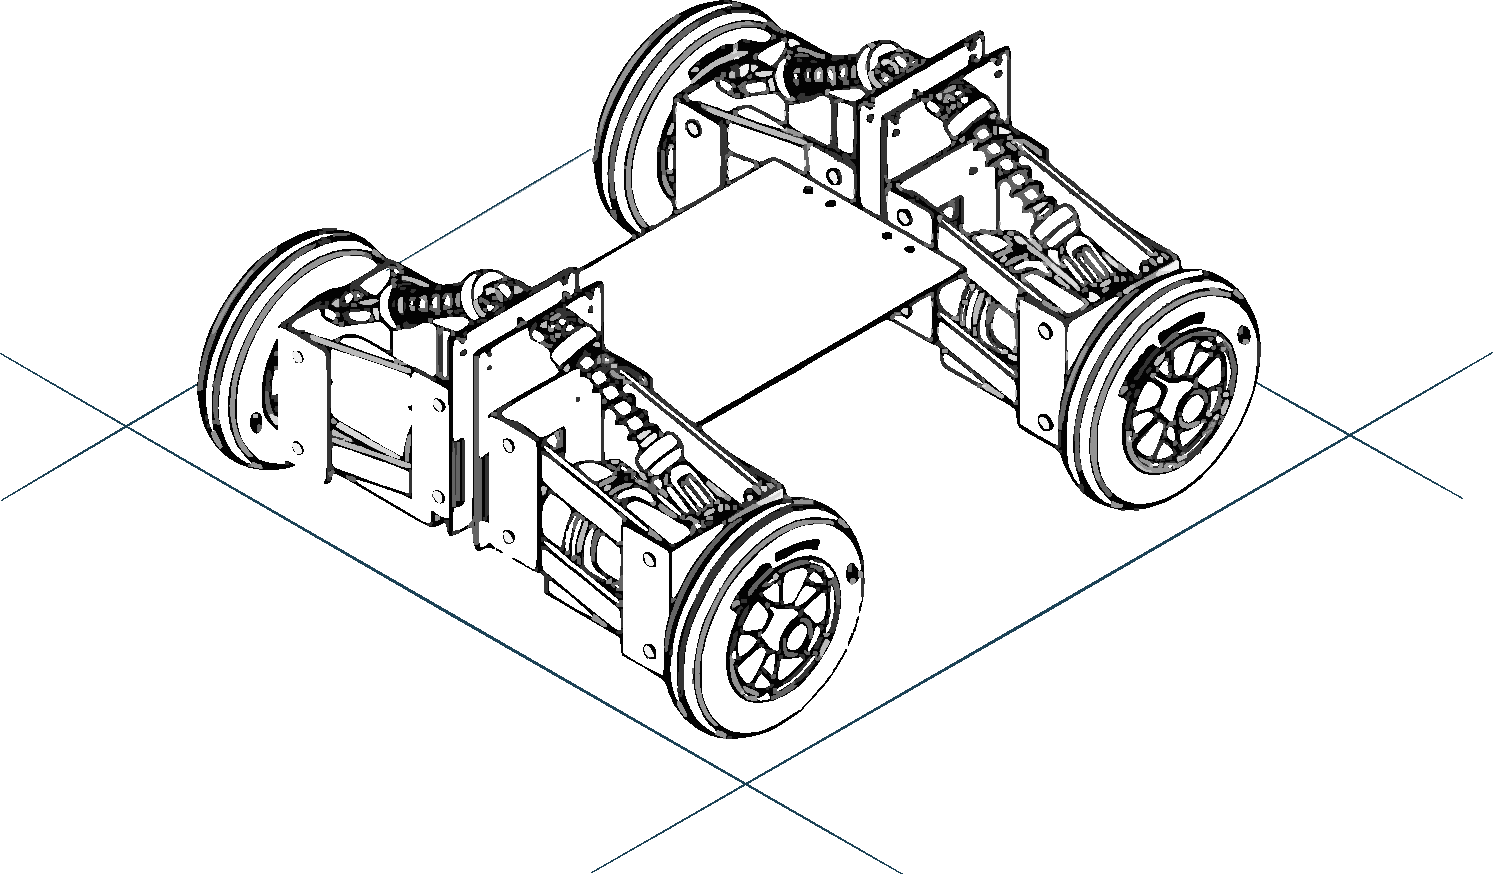
\includegraphics[width=0.5\textwidth]{figures/trak_skeleton}
\caption[Including an image with \texttt{\textbackslash includegraphics}]{A nice picture of something technical.}
\label{fig:trak}
\end{figure}

\section{Multi-Figures}
If you want to include several plots in one figure, use the \texttt{subfigure} environment within a \texttt{figure} environment. The subcaption package providing this environment is similar to subfig and subfigure, but comes with more flexibility and is a bit more intuitive. An example is given in Figure \ref{fig:options}, which also demonstrates the different options of the \texttt{\textbackslash includegraphics} command, like scaling, trimming, or rotating images. When you create a subfigure, make sure to use the \texttt{[b]} option which aligns the image on the bottom of its subfigure container: \texttt{\textbackslash begin\{subfigure\}\textbf{[b]}\{<widht>\}}. The necessary argument \texttt{<width>} specifies how big the ``containter'' for the image should be. 

Note that if the subcaptions of adjacent images span different numbers of lines they will not be aligned vertically (cf. Figs. \ref{fig:trim} and \ref{fig:smush} or Figs. \ref{fig:angle} and \ref{fig:draft}). In order to circumvent this issue you can use the alternative subcaption command \texttt{\textbackslash subcaptionbox[<list entry>]\{<heading>\}[<width>][<inner-pos>]\{<contents>\}} instead, which aligns captions at the top. An example is shown in Figure \ref{fig:capbox} -- compare the caption alignment of Figures \ref{fig:angle} and \ref{fig:draft} with Figures \ref{fig:angle2} and \ref{fig:draft2}.

\begin{figure}
\centering
\begin{subfigure}[b]{.3\linewidth}
	\centering
	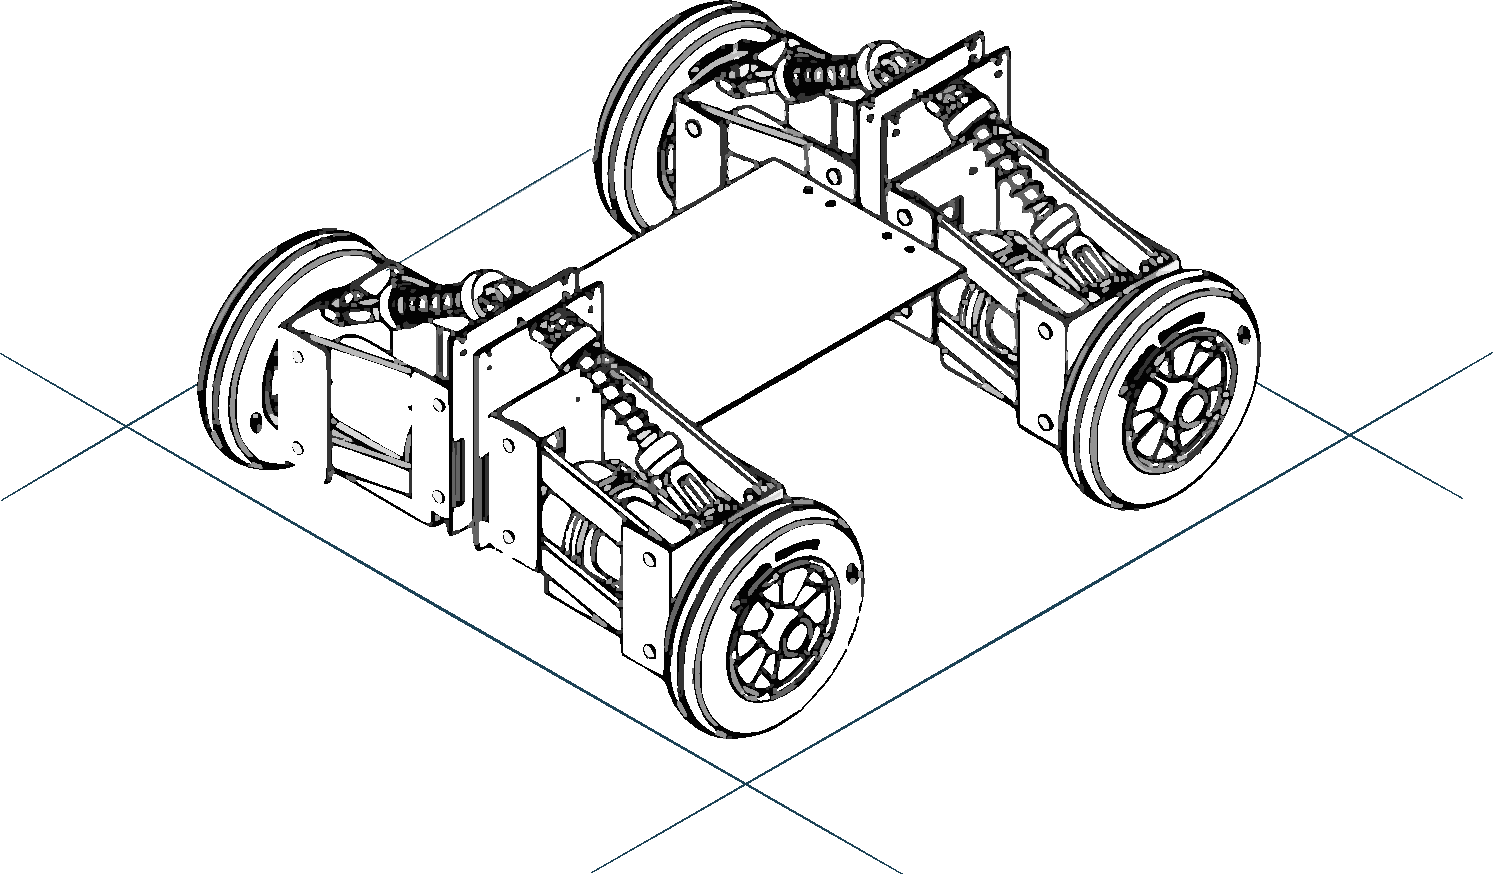
\includegraphics[scale=0.2,trim={3cm 2cm 4cm 0},clip]{figures/trak_skeleton}
	\caption{Options: scale=0.2, trim= \{3cm 2cm 4cm 0\}, clip.}
	\label{fig:trim}
\end{subfigure}\hfill
\begin{subfigure}[b]{.65\linewidth}
	\centering
	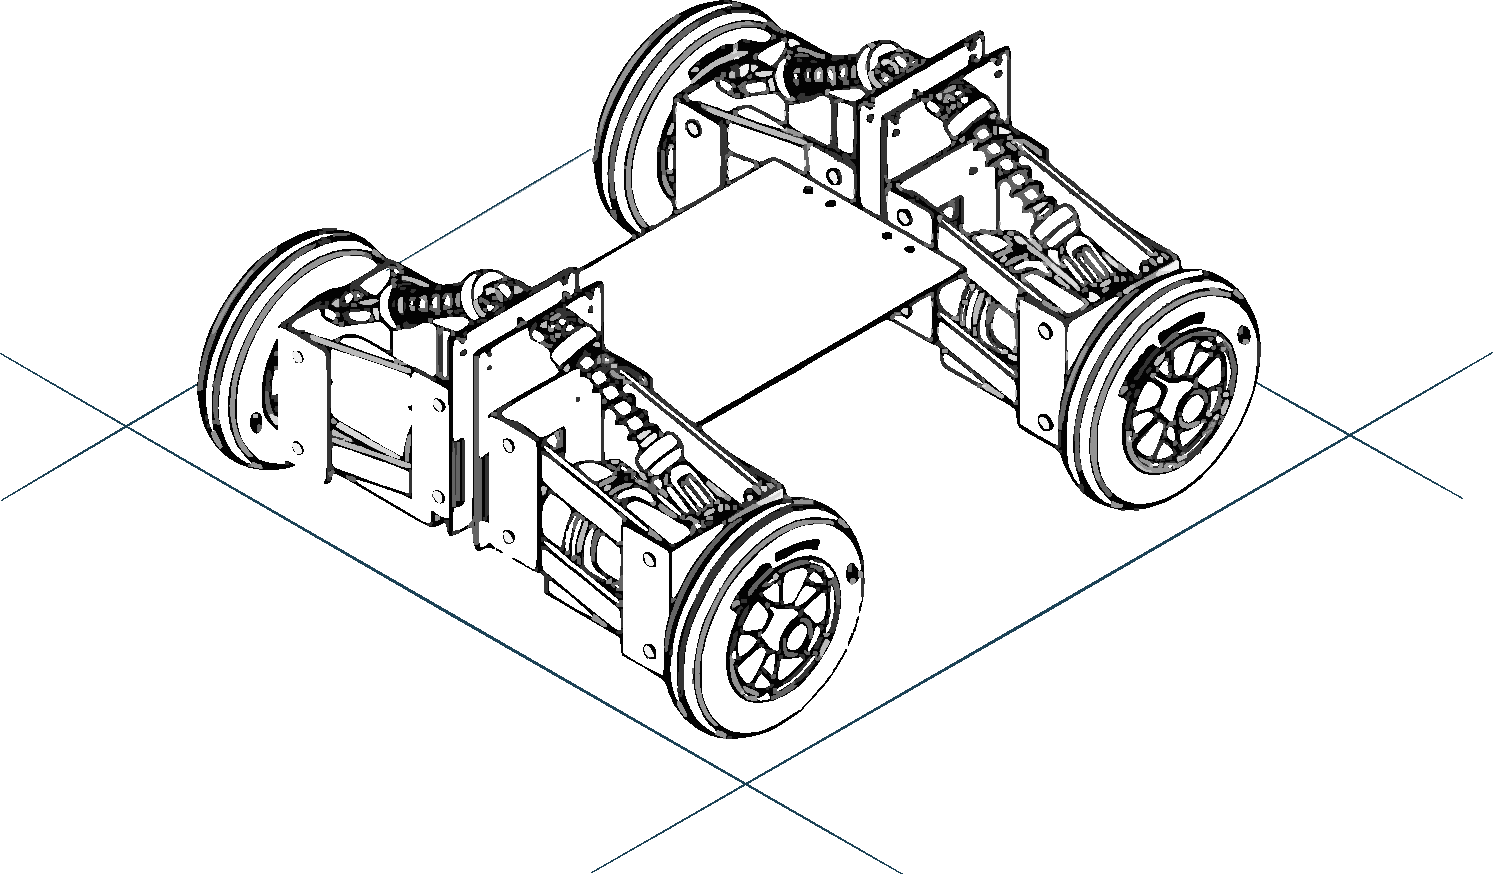
\includegraphics[width=\textwidth, height=2cm]{figures/trak_skeleton}
	\caption{Options: width=\textbackslash textwidth, height=2cm.}
	\label{fig:smush}
\end{subfigure}
\begin{subfigure}[b]{.45\linewidth}
	\centering
	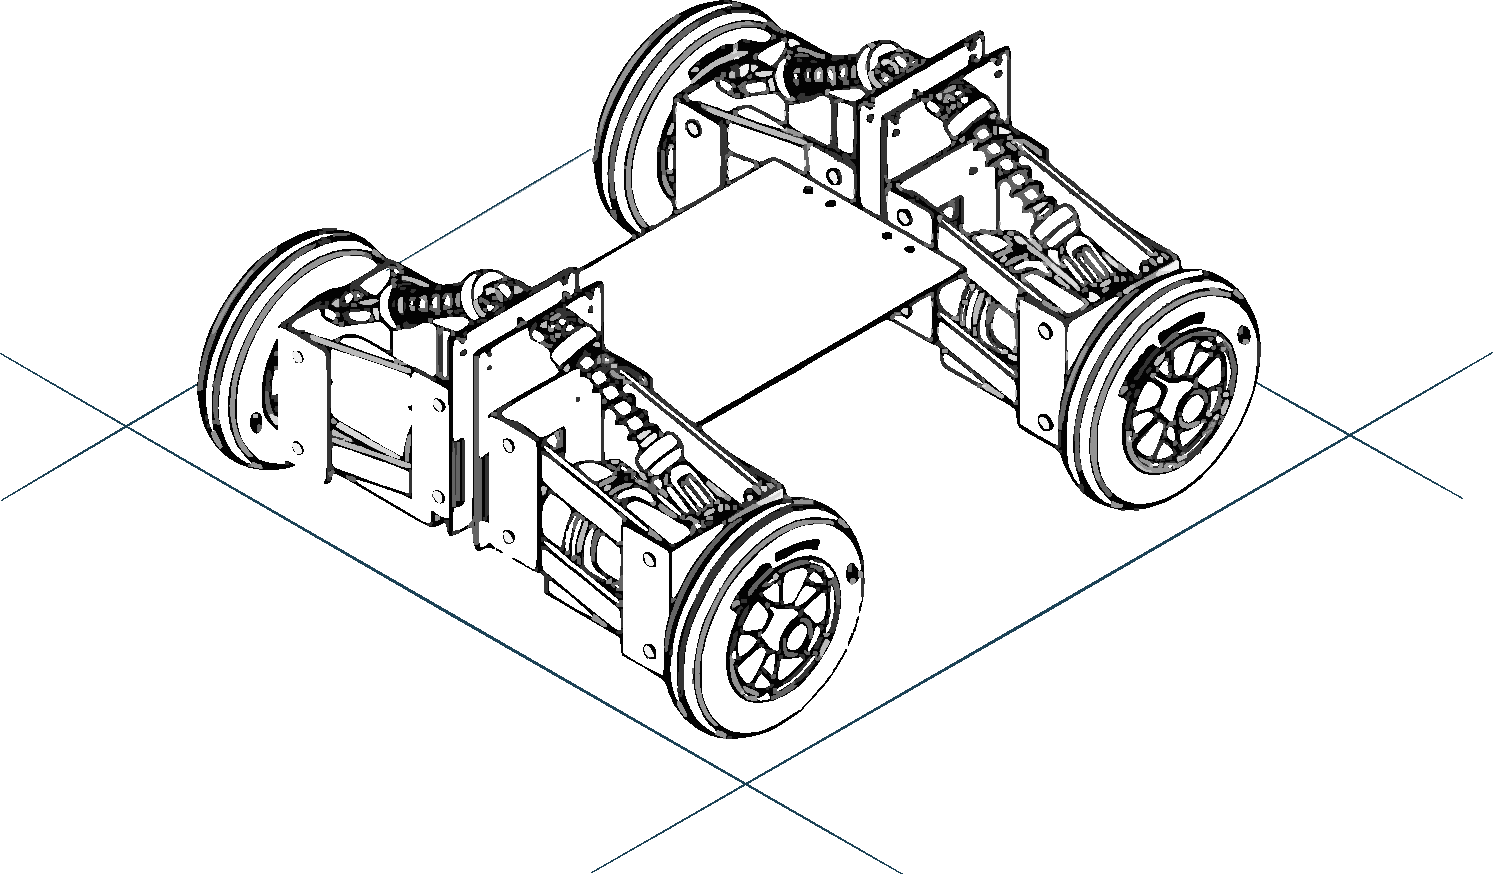
\includegraphics[width=5cm, angle=45]{figures/trak_skeleton}
	\caption{Options: width=5cm, angle=45.}
	\label{fig:angle}
\end{subfigure}\hfill
\begin{subfigure}[b]{.45\linewidth}
	\centering
	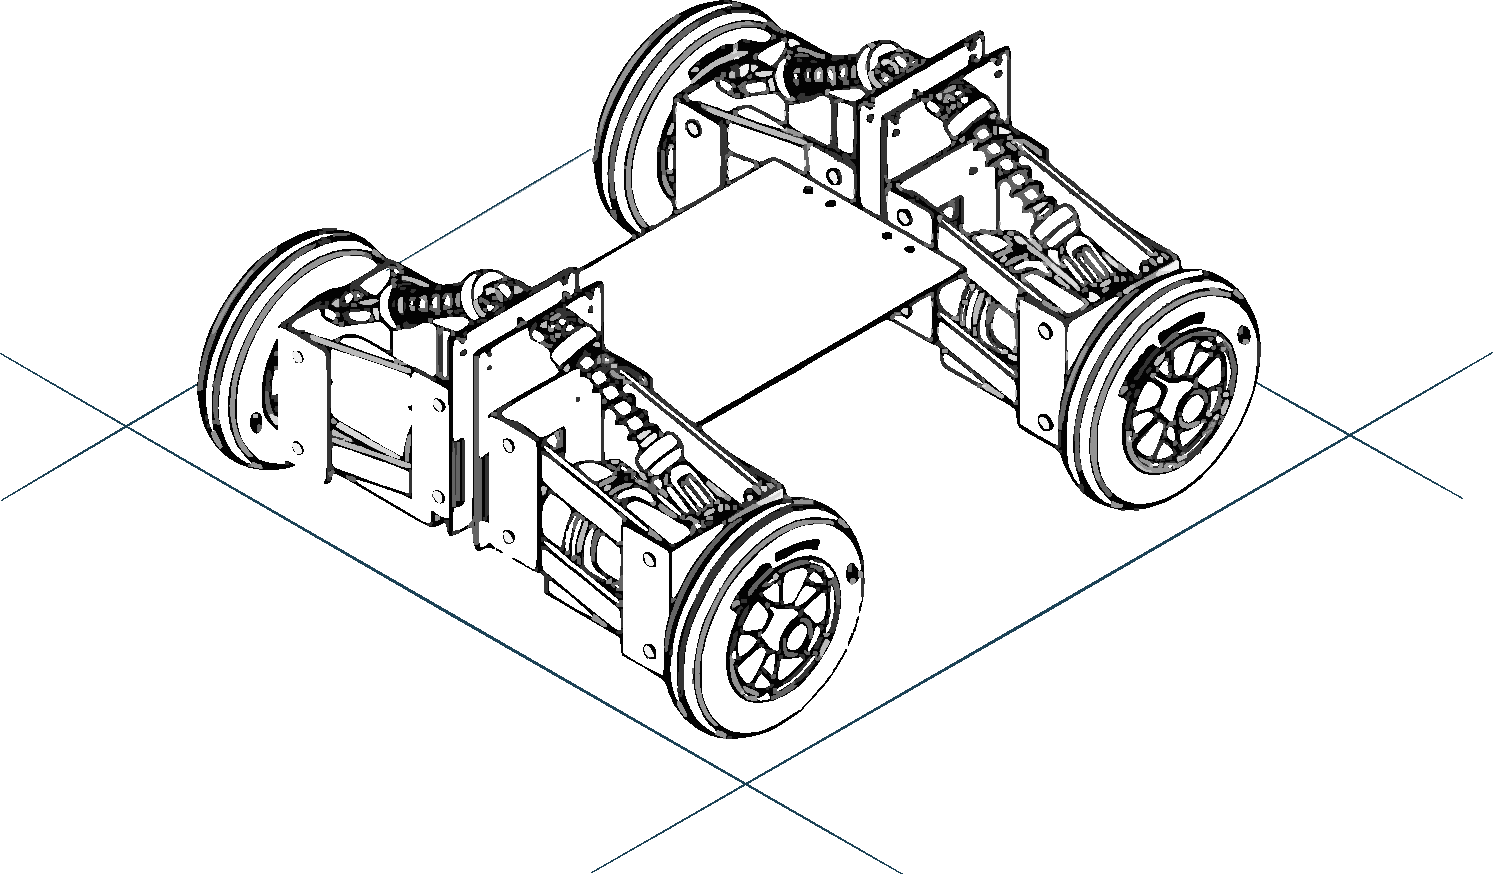
\includegraphics[draft, scale=0.25]{figures/trak_skeleton}
	\caption{Options: draft, scale=0.25. And this is some dummy text.}
	\label{fig:draft}
\end{subfigure}
\caption[Options of \texttt{\textbackslash includegraphics} and the \texttt{subfigure} environment]{Different options for the \texttt{\textbackslash includegraphics} command.}
\label{fig:options}
\end{figure}

\begin{figure}[H]
\centering
\subcaptionbox{Options: width=5cm, angle=45.\label{fig:angle2}}[.45\linewidth][c]{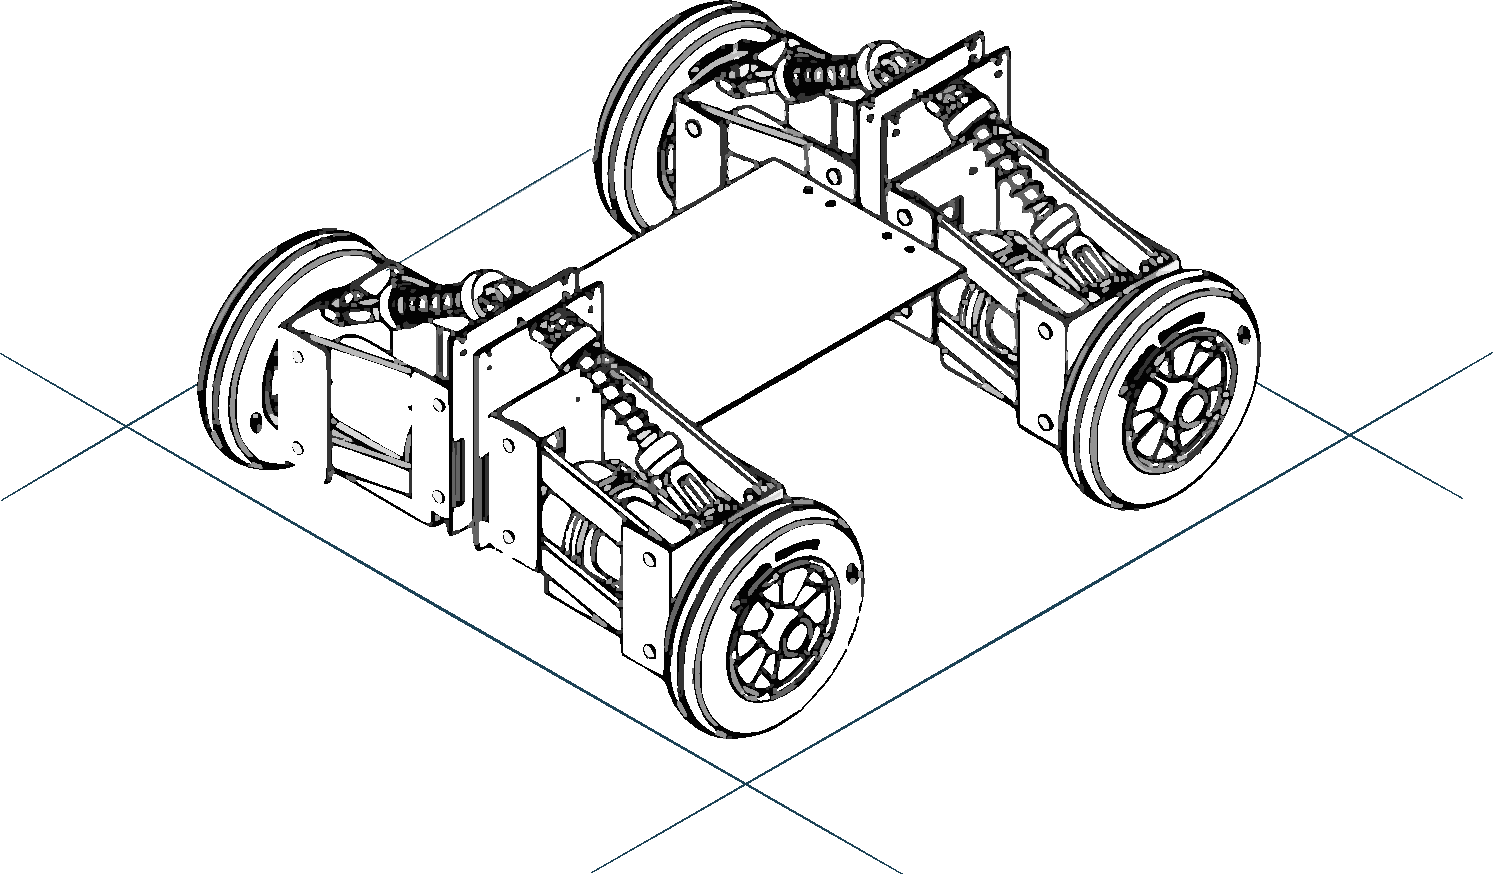
\includegraphics[width=5cm, angle=45]{figures/trak_skeleton}}
\hfill
\subcaptionbox{Options: draft, scale=0.25. And this is some dummy text.\label{fig:draft2}}[.45\linewidth][c]{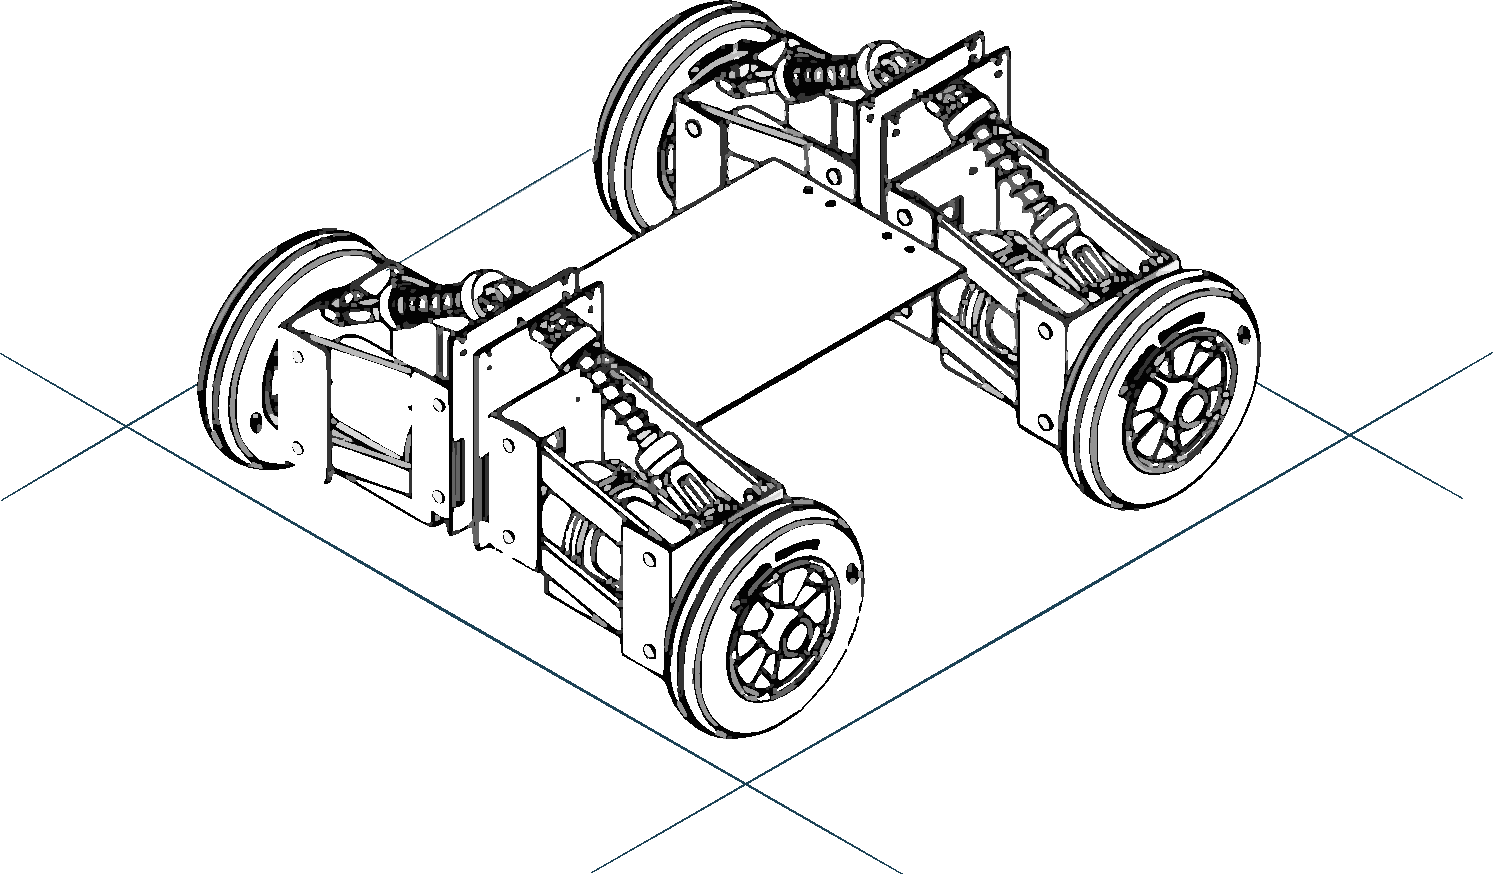
\includegraphics[draft, scale=0.25]{figures/trak_skeleton}}
\caption[\texttt{\textbackslash subcaptionbox} for multi-figures]{Effect of using \texttt{\textbackslash subcaptionbox}: All adjacent captions are aligned at the top, even if they span multiple lines.}
\label{fig:capbox}
\end{figure}


